\section{Introduzione}\label{intro}

Gli articoli scientifici sono materiale continuamente letto, richiesto e aggiornato in ambito universitario. Per questo motivo risulta interessante lo studio di funzionalità per estrarre i metadati da essi. Per metadati si intende l'informazione che descrive l'insieme di descrittori del pdf quali: titolo, autore, bibliografia, tematica.\\ In teoria il pdf avrebbe uno standard predefinito per la memorizzazione di metadati, ma l'eterogeneità dei tool di generazione PDF fa si che non venga rispettato; inoltre ci sono metadati come la bibliografia che non sono contemplati dallo standard. Per questo motivo si è reso necessario costruire un metodo che analizzasse a livello testuale il pdf e li estrapolasse.\\
Durante l'esame del corso di \textit{Data Base II} è stato studiato il processo di Information Retrieval al fine di estrarre metadati e come correlarli con i documenti in una biblioteca digitale come ad esempio Greenstone. Purtroppo come detto precentemente, l'estrazione dei metadati non è una cosa automatizzata e standardizzata ed è stato necessario elaborare un processo di analisi del testo del pdf, sfruttando le nozioni del corso; in questo senso l'elaborato si colloca come un approfondimento al corso per sviluppare un determinato senso critico a riguardo dell' Information Retrieval.\\
In particolare l'attenzione si è focalizza sulla bibliografia, visto che alcuni elaborati erano già stati effettuati su estrazione di titolo e autore da articoli scientifici \cite{Tarocchi}; i riferimenti bibliografici sono definiti come l'insieme dei riferimenti consultati e usati dall'autore per scrivere il suo articolo originale. In ogni articola alla fine si trova la lista dei riferimenti spesso accompagnata da una numerazione che abbina l'articolo alla parte citata nel testo. Un caso d'uso potrebbe essere quello in cui ad un lettore o ricercatore potrebbe risultare utile ottenere immediatamente dei riferimenti online relativi alla risorsa citata dall'articolo che sta leggendo per appronfondire una tematica. Perciò si è pensato ad un modo per estrarre la bibliografia dall' articolo e ottenere le risorse Web collegate a ciascuna voce, riportando dove presente sia il codice BibTex associato, che in alcuni casi, ove possibile, addirittura scaricarsi in locale l'articolo citato in formato PDF per consultarlo \textit{offline}.

E'facile capire come da un singolo articolo si crea una fitta rete di collegamenti ad altri articoli che a loro volta contengono altre citazioni. Risulta perciò interessante percorrere ricorsivamente l'intero grafo che collega l'un con l'altro i vari articoli. In questo senso sarebbe interessante provare a sviluppare un crwalter che dati in input una serie di articoli cerchi di indicizzare quelli che trova per collegamento, impostando una certa profondità di ricerca e costruirsi anche visivamente il grafo dei collegamenti degli articoli. Questa parte non è trattata nel nostro elaborato e sarà approfonita nella sezione degli sviluppi futuri.

In ultima analisi la bibliografia è un oggetto particolare che rappresenta il collante tra articoli che con molta probabilità condividono il medesimo tema di fondo; un esempio di bibliografia può essere quello riportato in Figura \ref{fig:ref-examples}, che presenta una precisa numerazione.\\

Nel seguito saranno spiegate nella sezione \ref{obiettivi} lo scopo e l'obiettivo dell'elaborato e i problemi citati nell'introduzione che ha permesso di risolvere. L'elaborato ha portato alla luce  un programma chiamato \textit{pdftoref} che ci occupa dell'estrazzione automatizzata dellla bibliografia. Nelle sezioni successive sarà spiegato come si è affronata l'analisi del problema, lo sviluppo dell'applicativo e infine i risultati ottenuti collegati alle conclusioni tratte.


\begin{figure}[htb]
\begin{center}
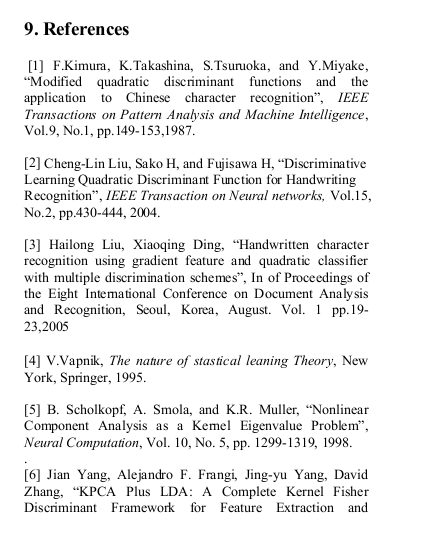
\includegraphics[scale=0.7]{ref.png}
\end{center}
\caption[Un esempio di bibliografia]{Un esempio di bibliografia estratte dall'articolo di una conferenza di ICDAR. E'subito intuitivo notare che la numerazione con parentesi quadre può costituire un ottimo punto di partenza per riuscire a capire quando inizia una nuova voce della bibliografia rispetto ad un'altra.}
\label{fig:ref-examples}
\end{figure}



